\begin{figure}[htbp]
\centering
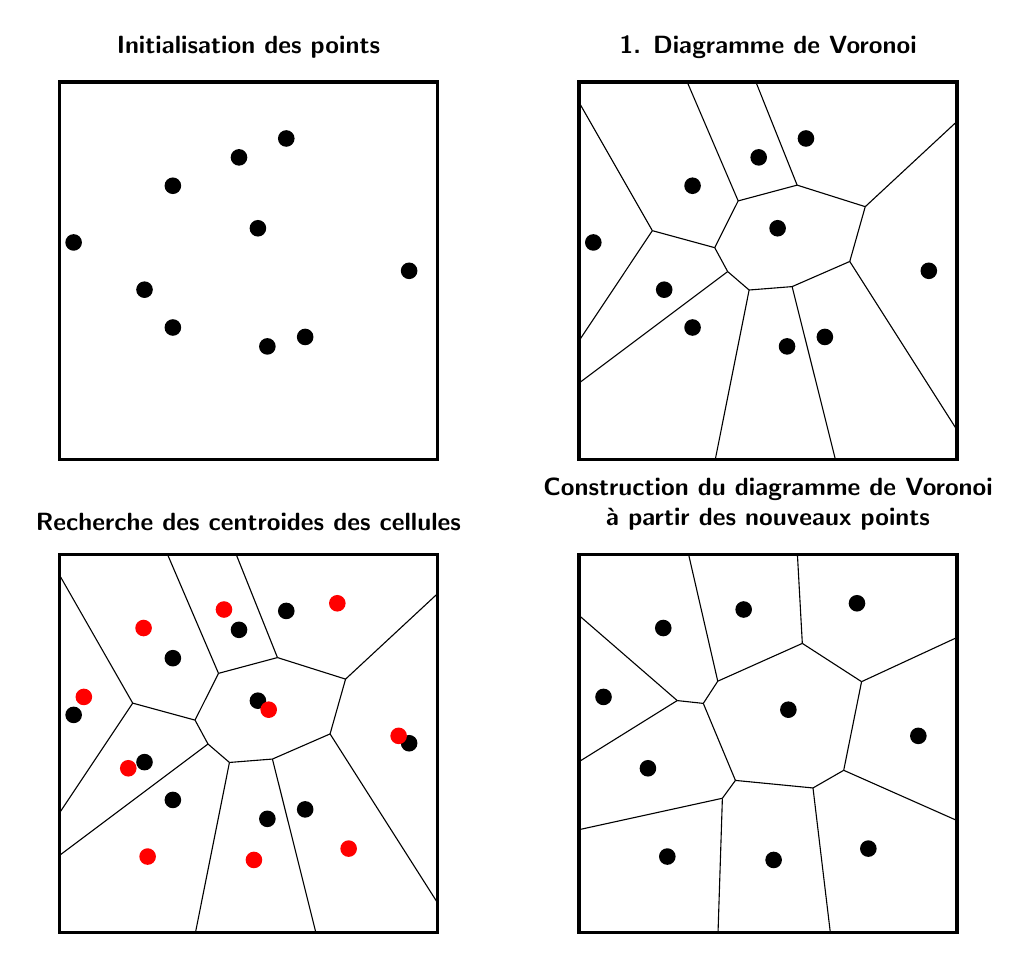
\begin{tikzpicture}[scale=1.2, every node/.style={scale=0.9}]

    % =================================================================
    % CARRÉ 1: Points Aléatoires
    % =================================================================
    \begin{scope}[shift={(0,0)}]
        % Le domaine (Carré)
        \draw[thick, line width=1.2pt] (0,0) rectangle (4,4);
        \node[above=6pt] at (2,4) {\textsf{\textbf{Initialisation des points}}};
        
        % Définition des coordonnées des germes
        \coordinate (A) at (0.15, 2.3);
        \coordinate (B) at (0.9, 1.8);
        \coordinate (C) at (1.2, 1.4);
        \coordinate (D) at (1.2, 2.9);
        \coordinate (E) at (1.9, 3.2);
        \coordinate (F) at (2.1, 2.45);
        \coordinate (G) at (2.2, 1.2);
        \coordinate (H) at (2.4, 3.4);
        \coordinate (I) at (2.6, 1.3);
        \coordinate (J) at (3.7, 2);
        
        % Dessin des points
        \foreach \p in {A,B,C,D,E,F,G,H,I,J} \fill (\p) circle (2.5pt);
        % \foreach \p in {A,B,C,D,E,F,G,H,I,J} \node[below=3pt] at (\p) {\textsf{\textbf{\p}}};
    \end{scope}

    % =================================================================
    % CARRÉ 2: Itération 0: construction du diagramme de voronoi
    % =================================================================
    \begin{scope}[shift={(5.5,0)}]
        % Le domaine
        \draw[thick, line width=1.2pt] (0,0) rectangle (4,4);
        \node[above=6pt] at (2,4) {\textsf{\textbf{1. Diagramme de Voronoi}}};
        
        % Même points
        \coordinate (A) at (0.15, 2.3);
        \coordinate (B) at (0.9, 1.8);
        \coordinate (C) at (1.2, 1.4);
        \coordinate (D) at (1.2, 2.9);
        \coordinate (E) at (1.9, 3.2);
        \coordinate (F) at (2.1, 2.45);
        \coordinate (G) at (2.2, 1.2);
        \coordinate (H) at (2.4, 3.4);
        \coordinate (I) at (2.6, 1.3);
        \coordinate (J) at (3.7, 2);
        
        % --- SEGMENTS DU DIAGRAMME DE VORONOI (33 segments générés) ---
        \draw[thin] (4.0, 0.314) -- (4.0, 3.582);
        \draw[thin] (4.0, 3.582) -- (4.0, 3.582);
        \draw[thin] (3.028, 2.679) -- (4.0, 3.582);
        \draw[thin] (2.864, 2.099) -- (4.0, 0.314);
        \draw[thin] (2.864, 2.099) -- (3.028, 2.679);
        \draw[thin] (4.0, 0.0) -- (4.0, 0.314);
        \draw[thin] (0.0, 0.0) -- (0.0, 0.813);
        \draw[thin] (4.0, 3.582) -- (4.0, 4.0);
        \draw[thin] (2.254, 1.833) -- (2.864, 2.099);
        \draw[thin] (1.683, 2.74) -- (2.307, 2.907);
        \draw[thin] (2.307, 2.907) -- (3.028, 2.679);
        \draw[thin] (1.435, 2.245) -- (1.683, 2.74);
        \draw[thin] (1.572, 1.992) -- (1.799, 1.797);
        \draw[thin] (1.435, 2.245) -- (1.572, 1.992);
        \draw[thin] (1.799, 1.797) -- (2.254, 1.833);
        \draw[thin] (1.143, 4.0) -- (1.87, 4.0);
        \draw[thin] (0.0, 4.0) -- (1.143, 4.0);
        \draw[thin] (1.87, 4.0) -- (4.0, 4.0);
        \draw[thin] (1.87, 4.0) -- (2.307, 2.907);
        \draw[thin] (1.143, 4.0) -- (1.683, 2.74);
        \draw[thin] (1.44, 0.0) -- (2.713, 0.0);
        \draw[thin] (1.44, 0.0) -- (1.799, 1.797);
        \draw[thin] (2.254, 1.833) -- (2.713, 0.0);
        \draw[thin] (2.713, 0.0) -- (4.0, 0.0);
        \draw[thin] (0.0, 0.0) -- (1.44, 0.0);
        \draw[thin] (0.0, 0.813) -- (1.572, 1.992);
        \draw[thin] (0.0, 3.781) -- (0.775, 2.425);
        \draw[thin] (0.0, 1.262) -- (0.775, 2.425);
        \draw[thin] (0.0, 1.262) -- (0.0, 3.781);
        \draw[thin] (0.0, 3.781) -- (0.0, 4.0);
        \draw[thin] (0.775, 2.425) -- (1.435, 2.245);
        \draw[thin] (0.0, 0.813) -- (0.0, 1.262);
        \draw[thin] (0.0, 1.262) -- (0.0, 1.262);

        \foreach \p in {A,B,C,D,E,F,G,H,I,J} \fill (\p) circle (2.5pt);
    \end{scope}

    % =================================================================
    % CARRÉ 3: centre des cellules
    % =================================================================
    \begin{scope}[shift={(0,-5)}]
        % Le domaine
        \draw[thick, line width=1.2pt] (0,0) rectangle (4,4);
        \node[above=6pt] at (2,4) {\textsf{\textbf{Recherche des centroides des cellules}}};
        
        % Même points
        \coordinate (A) at (0.15, 2.3);
        \coordinate (B) at (0.9, 1.8);
        \coordinate (C) at (1.2, 1.4);
        \coordinate (D) at (1.2, 2.9);
        \coordinate (E) at (1.9, 3.2);
        \coordinate (F) at (2.1, 2.45);
        \coordinate (G) at (2.2, 1.2);
        \coordinate (H) at (2.4, 3.4);
        \coordinate (I) at (2.6, 1.3);
        \coordinate (J) at (3.7, 2);
        
        % --- SEGMENTS DU DIAGRAMME DE VORONOI (33 segments générés) ---
        \draw[thin] (4.0, 0.314) -- (4.0, 3.582);
        \draw[thin] (4.0, 3.582) -- (4.0, 3.582);
        \draw[thin] (3.028, 2.679) -- (4.0, 3.582);
        \draw[thin] (2.864, 2.099) -- (4.0, 0.314);
        \draw[thin] (2.864, 2.099) -- (3.028, 2.679);
        \draw[thin] (4.0, 0.0) -- (4.0, 0.314);
        \draw[thin] (0.0, 0.0) -- (0.0, 0.813);
        \draw[thin] (4.0, 3.582) -- (4.0, 4.0);
        \draw[thin] (2.254, 1.833) -- (2.864, 2.099);
        \draw[thin] (1.683, 2.74) -- (2.307, 2.907);
        \draw[thin] (2.307, 2.907) -- (3.028, 2.679);
        \draw[thin] (1.435, 2.245) -- (1.683, 2.74);
        \draw[thin] (1.572, 1.992) -- (1.799, 1.797);
        \draw[thin] (1.435, 2.245) -- (1.572, 1.992);
        \draw[thin] (1.799, 1.797) -- (2.254, 1.833);
        \draw[thin] (1.143, 4.0) -- (1.87, 4.0);
        \draw[thin] (0.0, 4.0) -- (1.143, 4.0);
        \draw[thin] (1.87, 4.0) -- (4.0, 4.0);
        \draw[thin] (1.87, 4.0) -- (2.307, 2.907);
        \draw[thin] (1.143, 4.0) -- (1.683, 2.74);
        \draw[thin] (1.44, 0.0) -- (2.713, 0.0);
        \draw[thin] (1.44, 0.0) -- (1.799, 1.797);
        \draw[thin] (2.254, 1.833) -- (2.713, 0.0);
        \draw[thin] (2.713, 0.0) -- (4.0, 0.0);
        \draw[thin] (0.0, 0.0) -- (1.44, 0.0);
        \draw[thin] (0.0, 0.813) -- (1.572, 1.992);
        \draw[thin] (0.0, 3.781) -- (0.775, 2.425);
        \draw[thin] (0.0, 1.262) -- (0.775, 2.425);
        \draw[thin] (0.0, 1.262) -- (0.0, 3.781);
        \draw[thin] (0.0, 3.781) -- (0.0, 4.0);
        \draw[thin] (0.775, 2.425) -- (1.435, 2.245);
        \draw[thin] (0.0, 0.813) -- (0.0, 1.262);
        \draw[thin] (0.0, 1.262) -- (0.0, 1.262);

        % Option B: Geometric Centroids of the clipped cells
        \coordinate (CA) at (0.258, 2.49);
        \coordinate (CB) at (0.728, 1.735);
        \coordinate (CC) at (0.933, 0.801);
        \coordinate (CD) at (0.89, 3.219);
        \coordinate (CE) at (1.741, 3.415);
        \coordinate (CF) at (2.214, 2.355);
        \coordinate (CG) at (2.058, 0.765);
        \coordinate (CH) at (2.94, 3.481);
        \coordinate (CI) at (3.06, 0.885);
        \coordinate (CJ) at (3.589, 2.078);

        \foreach \p in {A,B,C,D,E,F,G,H,I,J} \fill (\p) circle (2.5pt);
        \foreach \p in {CA,CB,CC,CD,CE,CF,CG,CH,CI,CJ} \fill[red] (\p) circle (2.5pt);
    \end{scope}

    % =================================================================
    % CARRÉ 4: nouveau voronoi
    % =================================================================
    \begin{scope}[shift={(5.5,-5)}]
        % Le domaine
        \draw[thick, line width=1.2pt] (0,0) rectangle (4,4);
        \node[above=6pt, align=center] at (2,4) {
            \textsf{\textbf{Construction du diagramme de Voronoi}}\\ 
            \textsf{\textbf{à partir des nouveaux points}}
        };

        
        % Option B: Geometric Centroids of the clipped cells
        \coordinate (CA) at (0.258, 2.49);
        \coordinate (CB) at (0.728, 1.735);
        \coordinate (CC) at (0.933, 0.801);
        \coordinate (CD) at (0.89, 3.219);
        \coordinate (CE) at (1.741, 3.415);
        \coordinate (CF) at (2.214, 2.355);
        \coordinate (CG) at (2.058, 0.765);
        \coordinate (CH) at (2.94, 3.481);
        \coordinate (CI) at (3.06, 0.885);
        \coordinate (CJ) at (3.589, 2.078);

        % --- SEGMENTS DU DIAGRAMME DE VORONOI (28 segments générés) ---
        \draw[thin] (4.0, 0.0) -- (4.0, 1.182);
        \draw[thin] (2.475, 1.527) -- (2.658, 0.0);
        \draw[thin] (1.47, 0.0) -- (1.516, 1.418);
        \draw[thin] (1.654, 1.607) -- (2.475, 1.527);
        \draw[thin] (1.516, 1.418) -- (1.654, 1.607);
        \draw[thin] (2.8, 1.714) -- (4.0, 1.182);
        \draw[thin] (2.475, 1.527) -- (2.8, 1.714);
        \draw[thin] (0.0, 4.0) -- (1.158, 4.0);
        \draw[thin] (0.0, 1.086) -- (1.516, 1.418);
        \draw[thin] (2.31, 4.0) -- (2.362, 3.057);
        \draw[thin] (2.362, 3.057) -- (2.989, 2.652);
        \draw[thin] (2.31, 4.0) -- (4.0, 4.0);
        \draw[thin] (2.989, 2.652) -- (4.0, 3.12);
        \draw[thin] (4.0, 3.12) -- (4.0, 4.0);
        \draw[thin] (1.158, 4.0) -- (1.467, 2.657);
        \draw[thin] (1.467, 2.657) -- (2.362, 3.057);
        \draw[thin] (1.158, 4.0) -- (2.31, 4.0);
        \draw[thin] (1.314, 2.422) -- (1.467, 2.657);
        \draw[thin] (1.314, 2.422) -- (1.654, 1.607);
        \draw[thin] (2.8, 1.714) -- (2.989, 2.652);
        \draw[thin] (4.0, 1.182) -- (4.0, 3.12);
        \draw[thin] (0.0, 1.806) -- (0.0, 3.352);
        \draw[thin] (0.0, 1.806) -- (0.0, 1.806);
        \draw[thin] (0.0, 3.352) -- (1.038, 2.452);
        \draw[thin] (0.0, 1.806) -- (1.038, 2.452);
        \draw[thin] (0.0, 3.352) -- (0.0, 4.0);
        \draw[thin] (0.0, 1.446) -- (0.0, 1.806);
        \draw[thin] (1.038, 2.452) -- (1.314, 2.422);

        \foreach \p in {CA,CB,CC,CD,CE,CF,CG,CH,CI,CJ} \fill (\p) circle (2.5pt);
    \end{scope}


\end{tikzpicture}
\caption{Processus de génération du maillage dual de Voronoi à partir d'un nuage de points.}
\end{figure}
